\documentclass{beamer}
%\documentclass[xcolor={dvipsnames}, handout]{beamer} %for printing
\usepackage{haziq_beamer}
\bibliography{bib/phd-presentation-3}
\begin{document}

%%%%%%%%%%%%%%%%%%%%%%%%%%%%%%%%%%%%%%%%%%%%%%%%%%%%%%%%%%%%%%%%%%%%%%%%%%%%%%%%
%%% TITLE %%%%%%%%%%%%%%%%%%%%%%%%%%%%%%%%%%%%%%%%%%%%%%%%%%%%%%%%%%%%%%%%%%%%%%
%%%%%%%%%%%%%%%%%%%%%%%%%%%%%%%%%%%%%%%%%%%%%%%%%%%%%%%%%%%%%%%%%%%%%%%%%%%%%%%%

\title[I-prior probit]{Binary probit regression with I-priors}
\author[Haziq Jamil]{\large{Haziq Jamil}\\ \footnotesize{Supervisors: Dr. Wicher Bergsma \& Prof. Irini Moustaki}}
\institute[http://haziqj.ml]{Social Statistics (Year 3)\\ London School of Economics \& Political Science}
\date[8-9 May 2017]{8-9 May 2017\\
\hspace{1cm}\\
PhD Presentation Event\\
\hspace{1cm}\\
\href{http://haziqj.ml}{\color{fu-red} \textbf{http://haziqj.ml}}
}

\begin{frame}[plain]
  \addtocounter{framenumber}{-1}
  \titlepage
\end{frame}

%%%%%%%%%%%%%%%%%%%%%%%%%%%%%%%%%%%%%%%%%%%%%%%%%%%%%%%%%%%%%%%%%%%%%%%%%%%%%%%%
%%% TOC %%%%%%%%%%%%%%%%%%%%%%%%%%%%%%%%%%%%%%%%%%%%%%%%%%%%%%%%%%%%%%%%%%%%%%%%
%%%%%%%%%%%%%%%%%%%%%%%%%%%%%%%%%%%%%%%%%%%%%%%%%%%%%%%%%%%%%%%%%%%%%%%%%%%%%%%%

\mytoc

%%%%%%%%%%%%%%%%%%%%%%%%%%%%%%%%%%%%%%%%%%%%%%%%%%%%%%%%%%%%%%%%%%%%%%%%%%%%%%%%
%%% BODY %%%%%%%%%%%%%%%%%%%%%%%%%%%%%%%%%%%%%%%%%%%%%%%%%%%%%%%%%%%%%%%%%%%%%%%
%%%%%%%%%%%%%%%%%%%%%%%%%%%%%%%%%%%%%%%%%%%%%%%%%%%%%%%%%%%%%%%%%%%%%%%%%%%%%%%%

\section{Introduction}
\subsection{I-priors}

\begin{frame}{The regression model}
  \vspace{-5pt}
  \begin{itemize}\setlength\itemsep{1em}
    \item For $i = 1, \dots, n$, consider the regression model
    \begin{align*}
      \begin{gathered}
        y_i = f(x_i) + \epsilon_i \\
        (\epsilon_1, \dots, \epsilon_n) \sim \N(\bzero, \bPsi^{-1})
      \end{gathered}
    \end{align*}
    where $f \in \cF$, $y_i \in \bbR$, and $x_i = (x_{i1}, \dots, x_{ip}) \in \cX$.
  \end{itemize}
  \begin{center}
    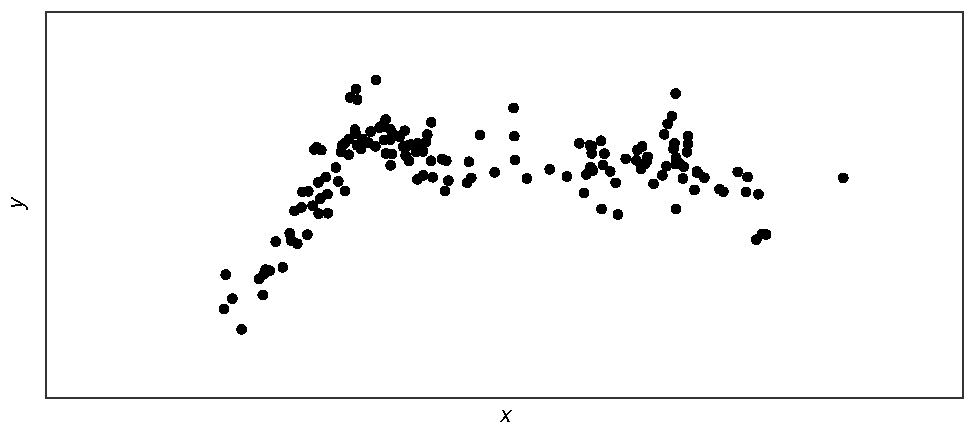
\includegraphics[scale=0.7]{figure/points}
  \end{center}
\end{frame}

\begin{frame}{I-priors}
  \vspace{-16pt}
  \blfootnote{\fullcite{Bergsma2017}}  
  \begin{itemize}\setlength\itemsep{1em}
    \item Let $\cF$ be a reproducing kernel Hilbert space (RKHS) with reproducing kernel $h_\lambda: \cX \times \cX \rightarrow \bbR$. An I-prior on $f$ is
    \[
      \big(f(x_1), \dots, f(x_n)\big)^\top \sim \N\big(\bff_0, \cI(f)\big)
    \] 
    with $\bff_0$ a prior mean, and $\cI$ the Fisher information for $f$, given by
    \[
      \cI\big(f(x), f(x')\big) = \sum_{k=1}^n\sum_{l=1}^n \psi_{kl} h_\lambda(x,x_k) h_\lambda(x',x_l).
    \]
    \item The I-prior regression model for $i = 1,\dots,n$ becomes
    \begin{align*}
      \begin{gathered}
        y_i = f_0(x_i) + \sum_{k=1}^n h_\lambda(x_i, x_k)w_k + \epsilon_i \\
        (w_1, \dots, w_n) \sim \N(\bzero, \bPsi) \\
        (\epsilon_1, \dots, \epsilon_n) \sim \N(\bzero, \bPsi^{-1})
      \end{gathered}    
    \end{align*}
  \end{itemize}
\end{frame}

\begin{frame}{I-priors (cont.)}
  \blfootnote{\fullcite{Jamil2017}}  
  \begin{itemize}
    \item Of interest is the posterior of the function
    \[
      p(\bff | \by ) = \frac{p(\by | \bff) p(\bff)}{\int p(\by | \bff) p(\bff) \d\bff},
    \]
    and also the posterior predictive distribution
    \[
      p(\by^* | \by ) = \int p(\by^* | \by, \bff ) p(\bff | \by ) \d\bff.
    \]
    \item Estimation using EM algorithm or direct maximisation of the marginal likelihood $\log p(y)$.
    \item Fully Bayesian estimation also possible.
  \end{itemize}
\end{frame}

%\begin{frame}{Canonical/Linear RKHS}
%  \vspace{-5pt}
%  \only<1>{
%    \begin{center}
%      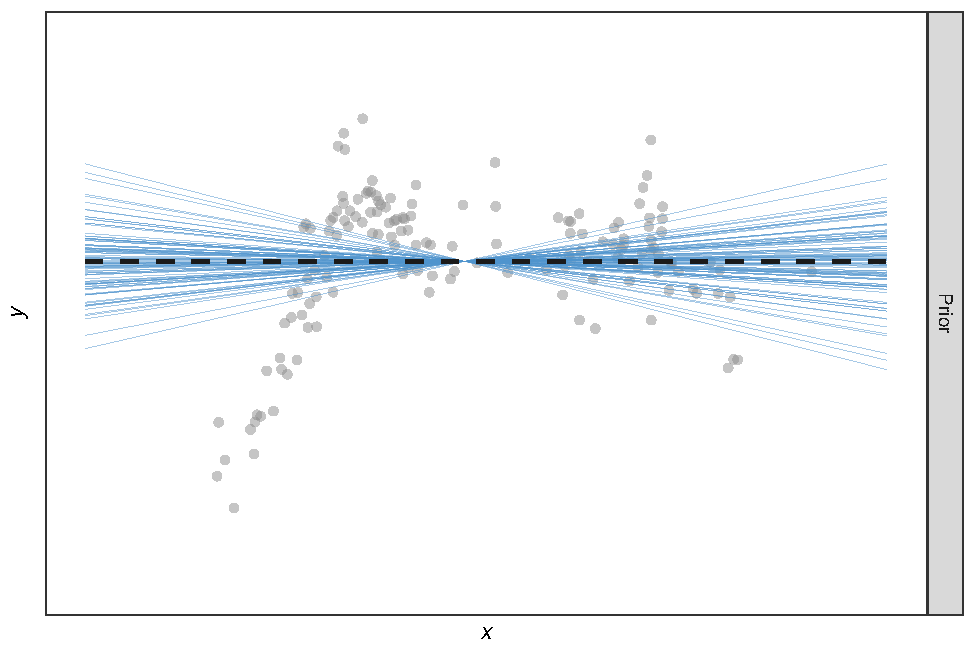
\includegraphics[scale=0.7]{figure/can-prior}
%    \end{center}
%  }
%  \only<2>{
%    \begin{center}
%      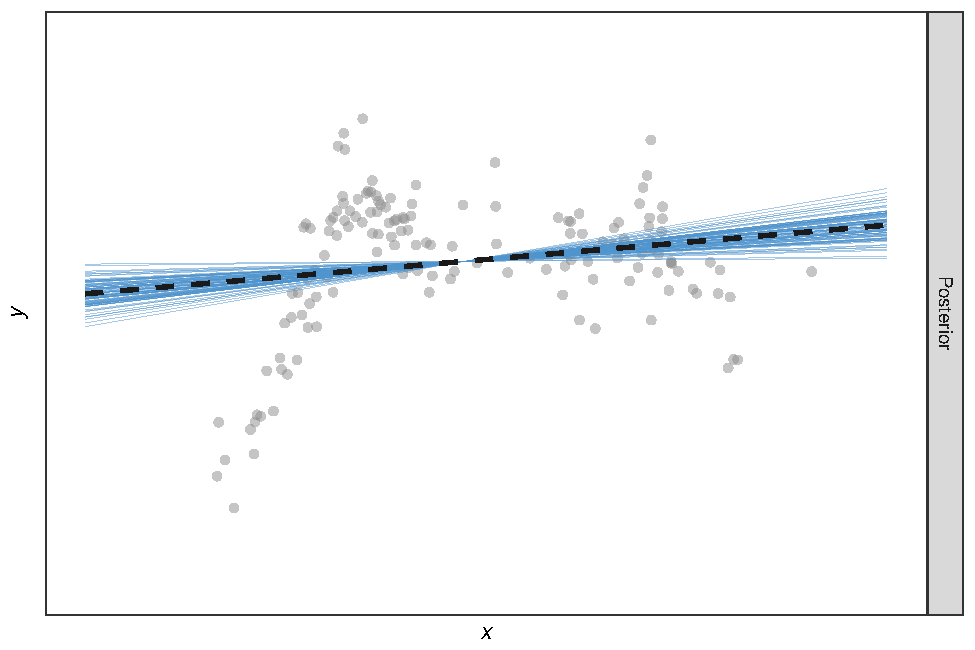
\includegraphics[scale=0.7]{figure/can-posterior}
%    \end{center}
%  }  
%\end{frame}

\begin{frame}{Fractional Brownian motion (FBM) RKHS}
  \vspace{-5pt}
  \only<1>{
    \begin{center}
      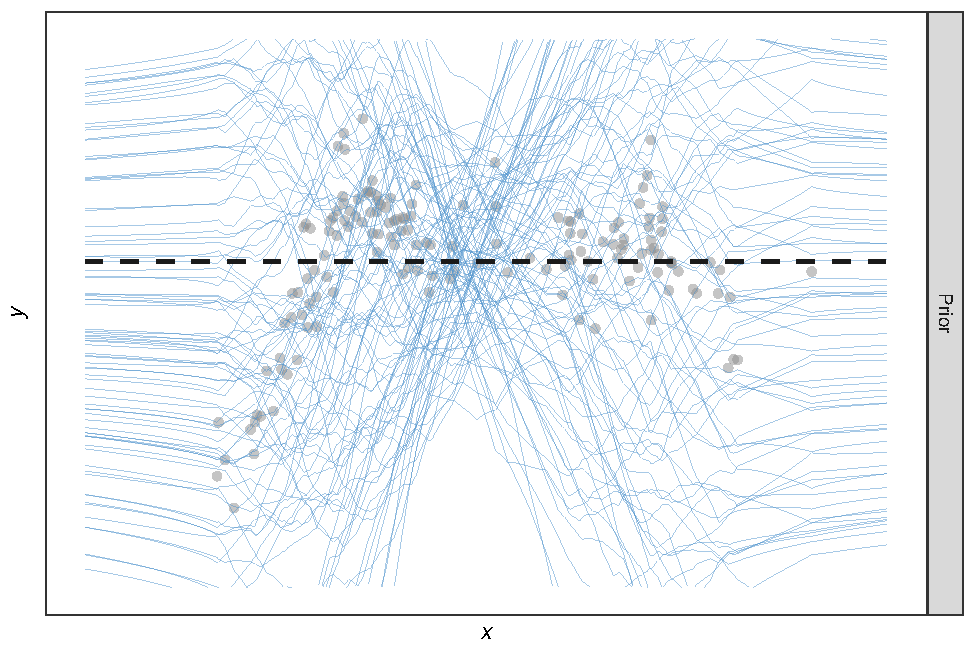
\includegraphics[scale=0.7]{figure/fbm-prior}
    \end{center}
  }
  \only<2>{
    \begin{center}
      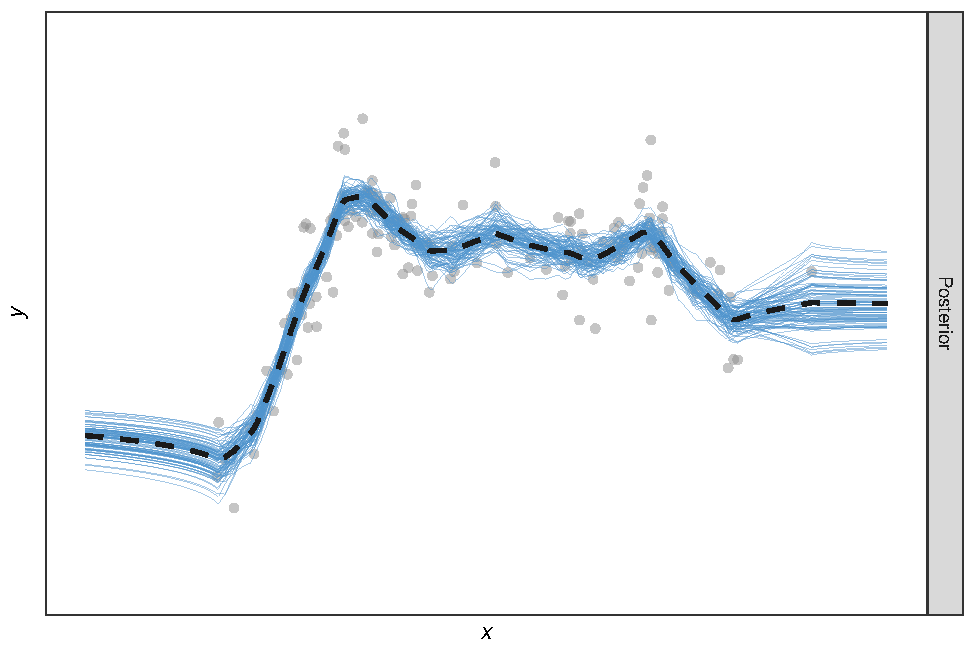
\includegraphics[scale=0.7]{figure/fbm-posterior}
    \end{center}
  }  
  \only<3>{
    \begin{center}
      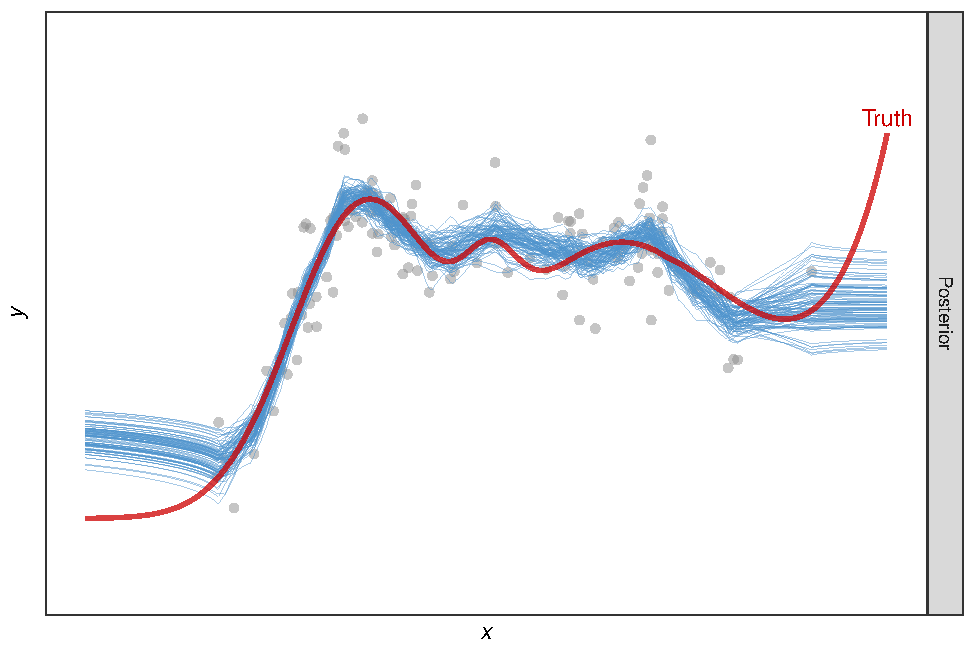
\includegraphics[scale=0.7]{figure/fbm-posterior-truth}
    \end{center}
  } 
\end{frame}

\begin{frame}{Posterior predictive distribution}
  \vspace{-5pt}
  \only<1>{
    \begin{center}
      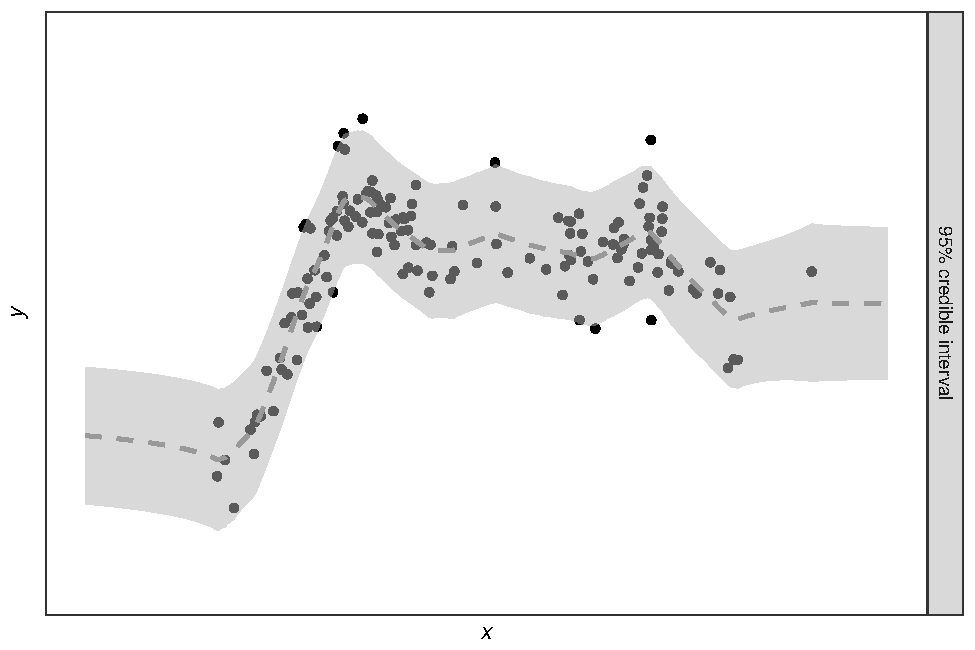
\includegraphics[scale=0.7]{figure/credible-interval}
    \end{center}
  }
  \only<2>{
    \begin{center}
      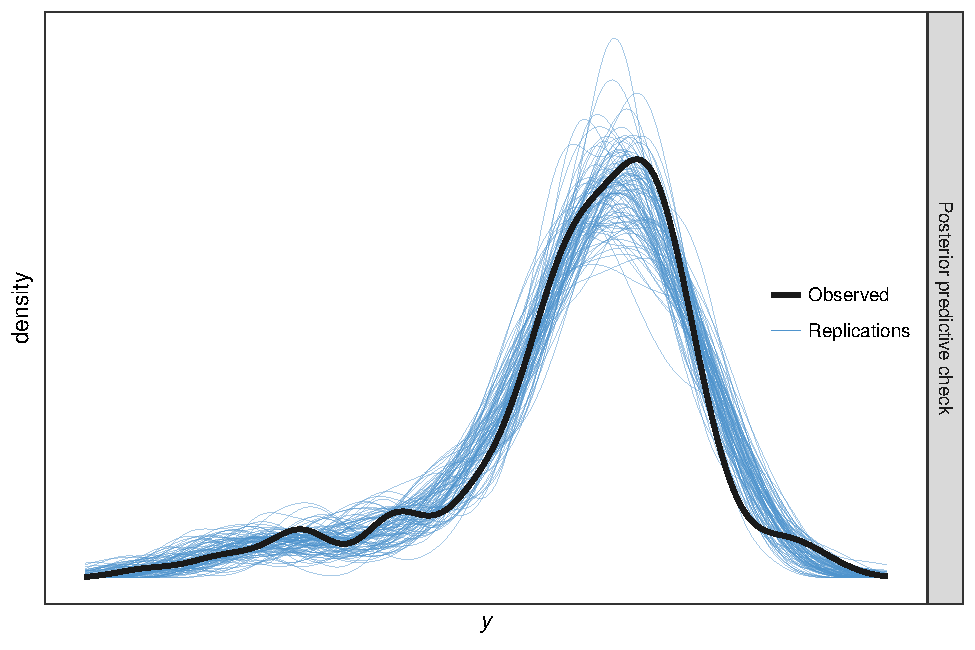
\includegraphics[scale=0.7]{figure/ppc}
    \end{center}
  }
\end{frame}

\subsection{PhD Roadmap}
\begin{frame}{Roadmap}
\end{frame}







\section[Probit I-prior]{Probit models with I-priors}
\transition
%\subsection{The latent variable motivation}

\begin{frame}{The latent variable motivation}
  \begin{itemize}
    \item Consider binary responses $y_1, \dots, y_n$ together with their corresponding covariates $x_1, \dots, x_n$. 
    \item For $i=1,\dots,n$, model the responses as
    \[
      y_i \sim \Bern(p_i).
    \]
    \item Assume that there exists continuous, underlying latent variables $y_1^*, \dots, y_n^*$, such that
    \[
      y_i =
      \begin{cases}
        1 & \text{ if } y_i^* \geq 0 \\
        0 & \text{ if } y_i^* < 0.    \\
      \end{cases}
    \]
    \item Model these continuous latent variables according to
    \[
      y_i^* = f(x_i) + \epsilon_i
    \]
    where $(\epsilon_1, \dots, \epsilon_n) \sim \N(\bzero, \bPsi^{-1})$ and $f \in \cF$ (some RKHS).
  \end{itemize}
\end{frame}

\subsection{Using I-priors}
\begin{frame}{Using I-priors}
  \begin{itemize}
    \item Assume an I-prior on $f$. Then,
    \begin{align*}
      \begin{gathered}
        f(x_i) = \alpha + \sum_{k=1}^n h_\lambda(x_i, x_k)w_k \\
        (w_1, \dots, w_n) \sim \N(\bzero, \bPsi) \\
      \end{gathered}
    \end{align*}
    \item For now, consider iid errors $\bPsi = \psi\bI_n$. In this case,
    \begin{align*}
      p_i = \Prob[y_i = 1] &= \Prob[y_i^* \geq 0] \\
      &= \Prob[\epsilon_i \leq f(x_i)] \\
      &= \Phi\Big(\psi^{1/2} ( 
%      {\color{gray} 
%      \underbrace{{\color{black} \alpha + {\textstyle\sum_{k=1}^n} h_\lambda(x_i, x_k)w_k}}_{\eta_i}
%      }
      \alpha + {\textstyle\sum_{k=1}^n} h_\lambda(x_i, x_k)w_k
      ) \Big)
    \end{align*}
    where $\Phi$ is the CDF of a standard normal.
    \item No loss of generality compared with using an arbitrary threshold $\tau$ or error precision $\psi$. Thus, set $\psi = 1$.
  \end{itemize}
\end{frame}

\begin{frame}{The probit I-prior model}
  \vspace{3pt}
  \begin{tikzpicture}[scale=1.1, transform shape]
    \tikzstyle{main}=[circle, minimum size = 10mm, thick, draw =black!80, node distance = 16mm]
    \tikzstyle{connect}=[-latex, thick]
    \tikzstyle{box}=[rectangle, draw=black!100]
      \node[main, draw=none] (fake) {};
      \node[main, fill = black!10] (H) [right=of fake, xshift=-1.65cm] {$x$};
      \node[main] (eta) [right=of H] {$f$};
      \node[main] (ystar) [right=of eta] {$y^*$};
      \node[main] (lambda) [above=of H, xshift=0.8cm, yshift=-0.5cm] {$\lambda$};
      \node[main] (alpha) [above=of eta, xshift=1.2cm, yshift=-0.5cm] {$\alpha$};  
      \node[main, fill = black!10] (y) [right=of ystar] {$y$};
      \node[main] (w) [below=of eta, yshift=0.5cm] {$w$};
    %  \node[main, fill = black!10] (x) [below=of eta,label=below:$x$] { };
      \path (alpha) edge [connect] (eta)
            (lambda) edge [connect] (eta)
    		(H) edge [connect] (eta) 
    		(eta) edge [connect] (ystar)
    		(ystar) edge [connect] (y)
    		(w) edge [connect] (eta);
      \path (H) edge [] node [above] {$h$} (eta);
      \node[rectangle, draw=black!100, fit= (H) (y) (w) ] {}; 
      \node[rectangle, fit= (w) (y), label=below right:N, xshift=1cm] {};  % the label
    \end{tikzpicture}
\end{frame}

\subsection{Estimation (and challenges)}

\begin{frame}{Estimation}
  \begin{columns}
    \uncover<1->{
    \begin{column}{0.47\textwidth}
      \vspace{6pt}
      \begin{itemize}\setlength\itemsep{0.5em}
        \item Denote $f_i = f(x_i)$ for short.
        \item The marginal density
        \vspace{4pt}
        \[
          \hspace{0.75cm} p(\by) = \int p(\by | \bff) p(\bff) \d\bff 
        \]
      \end{itemize}
    \end{column}}
    \uncover<4->{
    \begin{column}{0.5\textwidth}
    \vspace{-42pt}
      \begin{center}
        
\includegraphics[scale=0.40]{figure/taylor_expand_meme}
      \end{center}
    \end{column}}
  \end{columns}
  \uncover<1->{
  \vspace{-5pt}
  \[
    \phantom{p(\by)} = \int \prod_{i=1}^n \left[ \Phi(f_i)^{y_i} \big(1 - \Phi(f_i)\big)^{1-y_i} \right] \cdot \N(\alpha\bone_n, \bH_\lambda^2) \d\bff
  \]
  \hspace{0.65cm} for which $p(\bff|\by)$ depends, cannot be evaluated analytically.}
  \vspace{3pt}
  \begin{itemize}
    \item<2-> Some strategies:
    \begin{itemize}
      \item[\xmark]<2-> Naive Monte-Carlo integral
      \item[\xmark]<3-> EM algorithm with a MCMC E-step
      \item[{\color{FUorange}\cmark}]<4-> Laplace approximation
      \item[{\color{FUorange}\cmark}]<5-> MCMC sampling
    \end{itemize}
  \end{itemize}
\end{frame}

%\begin{frame}
%  \begin{center}
%    
\includegraphics[scale=0.5]{figure/taylor_expand_meme}
%  \end{center}
%\end{frame}

\subsection{What works}

\begin{frame}{Laplace's method}
  \blfootnote{\fullcite[§4.1, pp. 777-778.]{Kass1995}}
  \vspace{-15pt}
  \begin{itemize}\setlength\itemsep{0.8em}
    \item Interested in $p(\bff|\by) \propto p(\by|\bff)p(\bff) =: e^{Q(\bff)}$, with normalising constant $p(\by) = \int e^{Q(\bff)} \d\bff$. The Taylor expansion of $Q$ about its mode $\tilde\bff$
    \[
      Q(\bff) \approx Q(\tilde\bff) - \half (\bff - \tilde\bff)^\top\bA(\bff - \tilde\bff) 
    \]
    is recognised as the logarithm of an unnormalised Gaussian density, with $\bA = -\text{D}^2 Q(\bff)$ being the negative Hessian of $Q$ evaluated at  $\tilde\bff$.
    \item The posterior $p(\bff|\by)$ is approximated by $\N(\tilde\bff, \bA^{-1})$, and the marginal by
    \[
      p(\by) \approx (2\pi)^{n/2} \vert \bA \vert^{-1/2}  p(\by|\tilde\bff)p(\tilde\bff)
    \]
    \item Won't scale with large $n$; difficult to find modes in high dimensions.
  \end{itemize}
\end{frame}

\begin{frame}{Full Bayesian analysis using MCMC}
  \begin{itemize}\setlength\itemsep{0.5em}
    \item Assign hyperpriors on parameters of the I-prior, e.g.
    \begin{itemize}
      \item $\lambda^2 \sim \Gamma^{-1}(a,b)$
      \item $\alpha \sim \N(c,d^2)$
    \end{itemize}
    for a hierarchical model to be estimated fully Bayes.
    \item No closed-form posteriors - need to resort to MCMC sampling.
    \item Computationally slow, and sampling difficulty results in unreliable posterior samples.
  \end{itemize}
  *DENSITY PLOTS OF LAMBDA HERE*
\end{frame}










\section[Variational]{Variational inference}
\transition
\subsection{Introduction}

\begin{frame}{Variational inference}
  \blfootnote{\fullcite[Ch. 10]{Bishop2006}}
  \blfootnote{\fullcite[Ch. 21]{Murphy1991}}
  \vspace{-10pt}
  \begin{itemize}\setlength\itemsep{0.8em}
    \item Consider a statistical model where we have observations $(y_1, \dots, y_n)$ and also some latent variables $(z_1, \dots, z_n)$.
    \pause
    \item The $z_i$ could be random effects or some auxiliary latent variables.
    \item In a Bayesian setting, this could also include the parameters to be estimated.
    \pause
    \item \textbf{GOAL}: Find approximations for
    \begin{itemize}
      \item The posterior distribution $p(\bz|\by)$; and
      \item The marginal likelihood (or model evidence) $p(\by)$.
    \end{itemize}
    \item Variational inference is a deterministic approach, unlike MCMC.
  \end{itemize}
\end{frame}

\begin{frame}{Decomposition of the log marginal}  
  \vspace{-3pt}
  \begin{itemize}\setlength\itemsep{0.5em}
    \item Let $q(\bz)$ be some density function to approximate $p(\bz|\by)$. \pause Then the log-marginal density can be decomposed into
    \begin{align*}
      \log p(\by) &= \log p(\by,\bz) - \log p(\bz|\by) \\
      \onslide<3->{
      &= \int \left\{ \log \frac{p(\by,\bz)}{q(\bz)} - \log \frac{p(\bz|\by)}{q(\bz)} \right\} q(\bz) \d \bz \\    
      &=  \cL(q) +  \KL(q \Vert p) \\
      &\geq \cL(q) 
      }   
    \end{align*}
    \item<4-> $\cL$ is referred to as the ``lower-bound'', and it serves as a surrogate function to the marginal.
    \item<4-> Maximising $\cL(q)$ is equivalent to minimising $\KL(q \Vert p)$.
    \item<4-> Although $\KL(q \Vert p)$ is minimised at $q(\bz) \equiv p(\bz|\by)$ (c.f. EM algorithm), we are unable to work with $p(\bz|\by)$.
  \end{itemize}
\end{frame}

\begin{frame}{Comparison of approximations (density)}
  \vspace{-5pt}
  \only<1|handout:0>{
    \begin{center}
      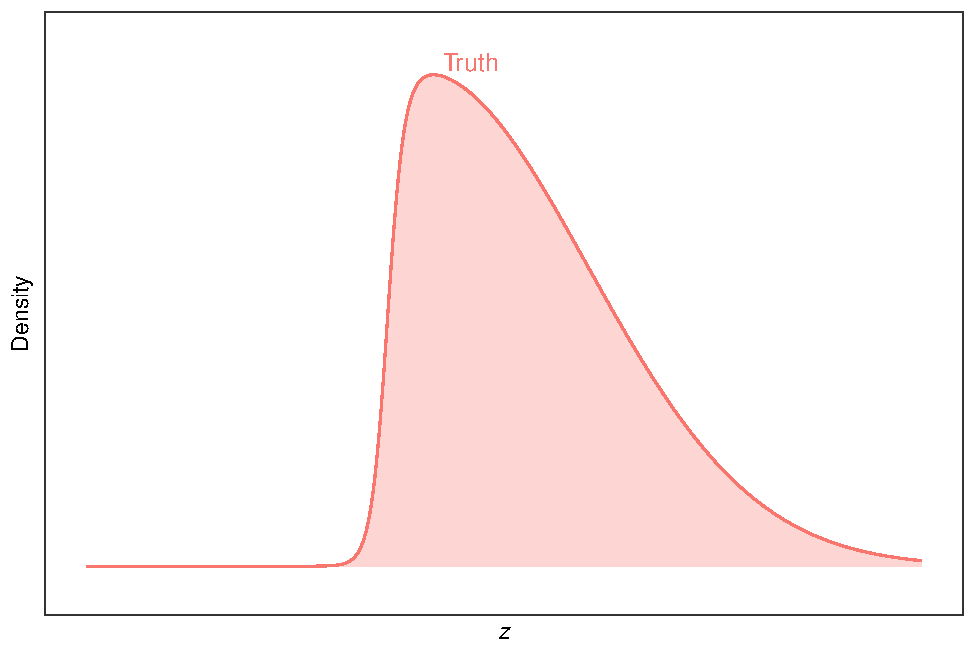
\includegraphics[scale=0.7]{figure/compare1}
    \end{center}
  }
%  \only<2|handout:0>{
%    \begin{center}
%      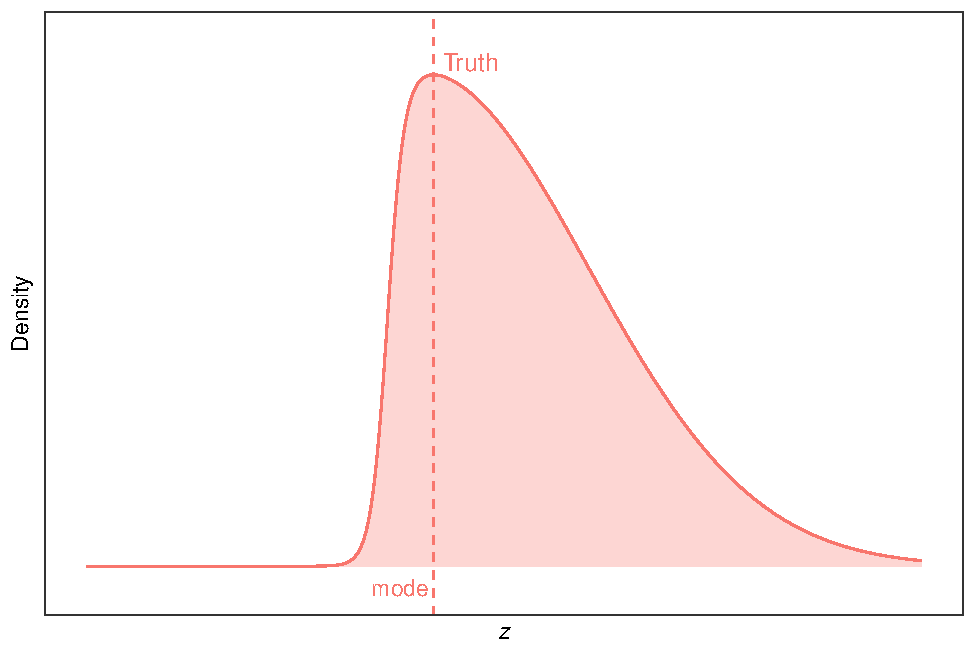
\includegraphics[scale=0.7]{figure/compare2}
%    \end{center}
%  }  
  \only<2|handout:0>{
    \begin{center}
      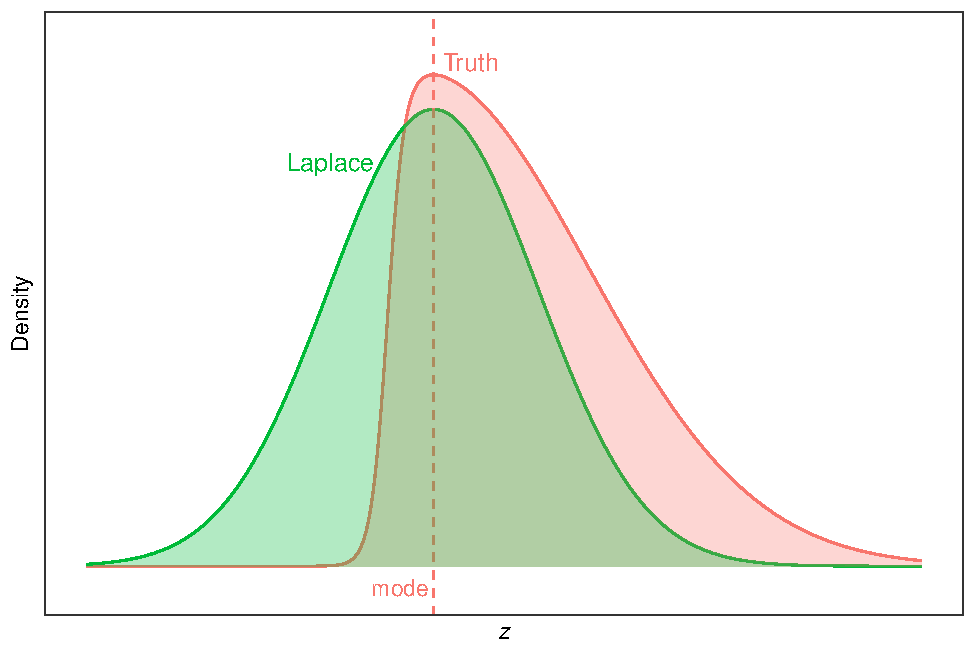
\includegraphics[scale=0.7]{figure/compare3}
    \end{center}
  } 
%  \only<4|handout:0>{
%    \begin{center}
%      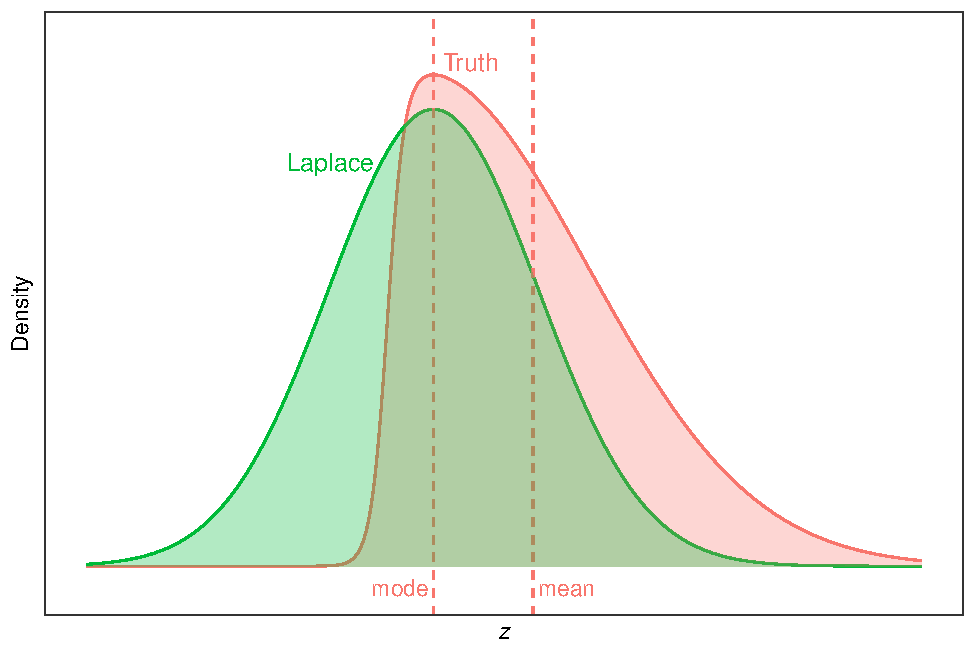
\includegraphics[scale=0.7]{figure/compare4}
%    \end{center}
%  } 
  \only<3|handout:1>{
    \begin{center}
      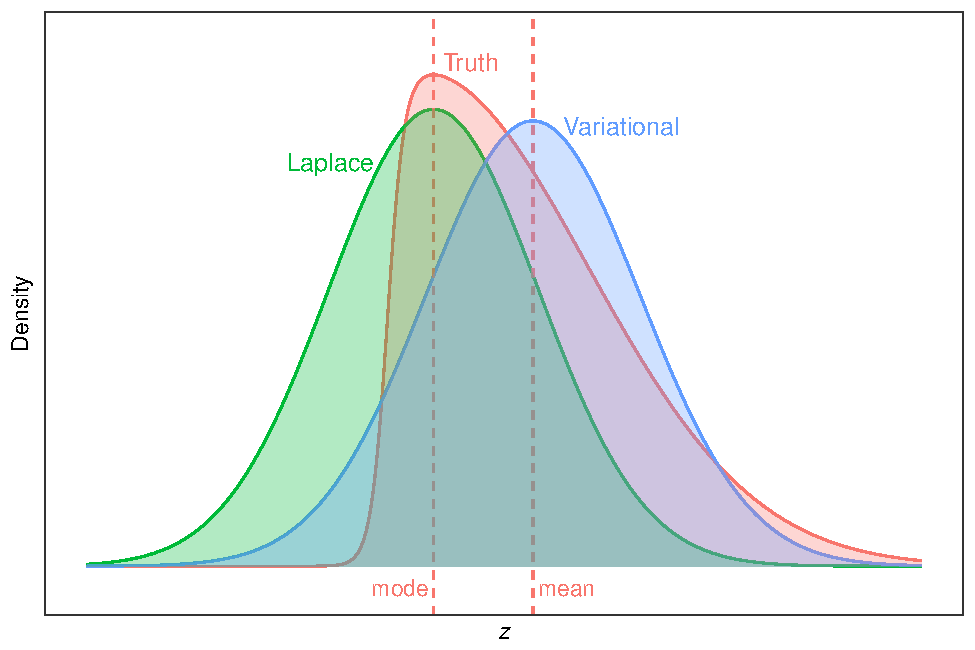
\includegraphics[scale=0.7]{figure/compare5}
    \end{center}
  } 
\end{frame}

\begin{frame}{Comparison of approximations (deviance)}
  \vspace{-5pt}
  \begin{center}
    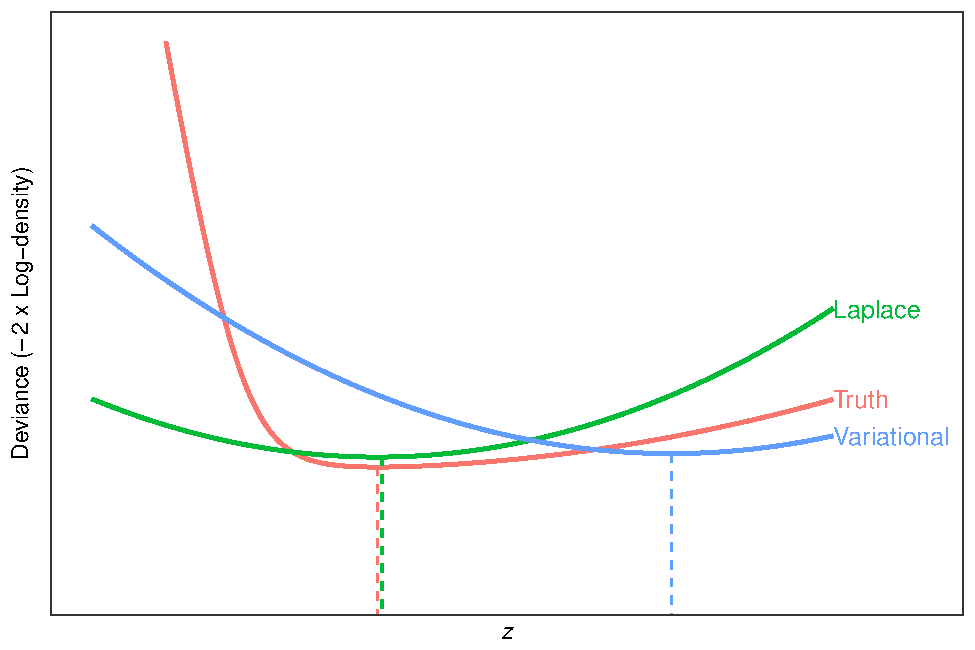
\includegraphics[scale=0.7]{figure/compare6}
  \end{center}
\end{frame}

\subsection{Mean-field factorisation}

\begin{frame}{Factorised distributions (Mean-field theory)}
  \blfootnote{\fullcite{Blei2016}}
  \vspace{-20pt}
  \begin{itemize}
    \item<1-> Maximising $\cL$ over all possible $q$ not feasible. Need some restrictions, but only to achieve tractability.
    \item<1-> Suppose we partition elements of $\bz$ into $m$ disjoint groups $\bz = (\bz^{(1)}, \dots, \bz^{(m)})$, and assume
    \[
      q(\bz) = \prod_{j=1}^m q_j(\bz^{(j)})
    \]
    \item<2-> Under this restriction, the solution to $\argmax_q \cL(q)$ is
    \begin{align}\label{eq:meanfieldsoln}
      \tilde q_j(\bz^{(j)}) \propto \exp\big(\E_{-j}[\log p(\by,\bz)]\big)
    \end{align}
    for $j \in \{1,\dots,m\}$.
    \item<3-> In practice, these unnormalised densities are of recognisable form (especially if conjugate priors are used).
    \vspace{4pt}
  \end{itemize}
\end{frame}

\begin{frame}[label=cavi]{Coordinate ascent mean-field variational inference (CAVI)}
  \vspace{-5pt}
  \begin{itemize}\setlength\itemsep{0.4em}
    \item The optimal distributions are coupled with another, i.e. each $\tilde q_j(\bz^{(j)})$ depends on the optimal moments of $\bz^{(k)}$, $k \in \{1,\dots,m:k \neq j\}$.
    \item One way around this to employ an iterative procedure.
    \item Assess convergence by monitoring the lower bound
    \[
      \cL(q) = \E_{ q}[\log p(\by, \bz)] - \E_{ q}[\log q(\bz)].
    \]
  \end{itemize}
  \vspace{-12pt}
    \begin{center}
    \scalebox{0.9}{
    \begin{minipage}{\linewidth}
  \begin{algorithm}[H]
    \caption{CAVI}\label{alg:cavi}
    \begin{algorithmic}[1]
      \State \textbf{initialise} Variational factors $q_j(\bz^{(j)})$
      \While{$\cL(q)$ not converged}
        \For{$j = 1,\dots,m$}
          \State $\log q_j(\bz^{(j)}) \gets \E_{-j}[\log p(\by,\bz)] + \const$
        \EndFor
        \State $\cL(q) \gets \E_{ q}[\log p(\by, \bz)] - \E_{ q}[\log q(\bz)]$
      \EndWhile
      \State \textbf{return} $\tilde q(\bz) = \prod_{j=1}^m \tilde q_j(\bz^{(j)})$ 
    \end{algorithmic}
  \end{algorithm}
      \end{minipage}%
    }
  \end{center}
  
  \begin{textblock*}{3cm}(.89\textwidth,1\textheight)%
    \hyperlink{varex}{\beamerbutton{example}}      
  \end{textblock*}
\end{frame}


\section{Illustration in R}
\transition
%\subsection{R/\texttt{iprobit}}

\begin{frame}{Variational I-prior probit}
  \begin{tikzpicture}[scale=1.1, transform shape]
    \tikzstyle{main}=[circle, minimum size = 10mm, thick, draw =black!80, node distance = 16mm]
    \tikzstyle{connect}=[-latex, thick]
    \tikzstyle{box}=[rectangle, draw=black!100]
      \node[main, draw=none] (fake) {};
      \node[main, fill = black!10] (H) [right=of fake, xshift=-1.65cm] {$x_i$};
      \node[main, double, double distance=0.6mm] (eta) [right=of H] {$f_i$};
      \node[main, draw=colpur] (ystar) [right=of eta] {\color{colpur} $y_i^*$};
      \node[main, draw=colblu] (lambda) [above=of H, xshift=0.4cm, yshift=-0.4cm] {\color{colblu} $\lambda$};  
      \node[main, draw=colgre] (alpha) [above=of eta, yshift=0.3cm] {\color{colgre} $\alpha$};  
      \node[main, fill = black!10] (y) [right=of ystar] {$y_i$};
      \node[main, draw=colred] (w) [below=of eta, yshift=0.4cm] {\color{colred} $w_i$};  
      \path (alpha) edge [connect] (eta)
            (lambda) edge [connect] (eta)
    		(H) edge [connect] (eta) 
    		(eta) edge [connect] (ystar)
    		(ystar) edge [connect] (y)
    		(w) edge [connect] (eta)
            (H) edge [] node [above] {$h$} (eta);
      \node[rectangle, draw=black!100, fit= (H) (y) (w) ] {}; 
      \node[rectangle, fit= (w) (y), label=below right:{$i=1,\dots,n$}, xshift=-0.35cm, yshift=0.55cm] {};  % the label
    \end{tikzpicture}
    
    \begin{textblock*}{0.48\textwidth}(0.52\textwidth,0.55cm)
    \begin{block}{}
    \vspace{-1.6em}
      \begin{align*}
        &p(\by,\by^*,\bw,\alpha,\lambda)  \\
        &= p(\by|\by^*)p(\by^*|\bff)p(\bw)p(\lambda)p(\alpha) \\
        &= {\textstyle\prod_{i=1}^n} \ind[y_i^* \geq 0]^{y_i} \ind[y_i^* < 0]^{1-y_i} \\
        &\phantom{==} \cdot {\color{colpur} {\textstyle\prod_{i=1}^n} \{ \N(f_i,1) \}} \cdot {\color{colred} [\N(0,1)]^n} \\
        &\phantom{==} \cdot {\color{colblu} \N(\lambda_0,\kappa_0^{-1})} \cdot  {\color{colgre} \N(\alpha_0,\tau_0^{-1})}
      \end{align*}
    \end{block}
  \end{textblock*}
\end{frame}

\begin{frame}{Posterior distribution}
  \begin{itemize}
    \item Approximate the posterior by a mean-field variational density
    \[
      p(\by^*,\bw,\alpha,\lambda|\by) \approx \prod_{i=1}^n q(y_i^*)q(\bw)q(\alpha)q(\lambda)\vspace{-2pt}
    \]
    where
  \end{itemize}
  \vspace{-15pt}
  \begin{center}   
    \begin{gather*}
      q(y_i^*) \equiv 
      \begin{cases}
        \ind[y_i^* \geq 0] \N(\tilde f_i, 1) &\text{ if } y_i = 1\\
        \ind[y_i^* < 0] \N(\tilde f_i, 1) &\text{ if } y_i = 0\\
      \end{cases}
    \hspace{1cm}
    q(\bw) \equiv \N(\tilde\bw, \tilde\bV_w) \\[0.5em]
    q(\lambda) \equiv \N(\tilde\lambda, \tilde v_w)
    \hspace{1cm}  
    q(\alpha) \equiv \N(\tilde\alpha,1/n) \\[0.5em]
    \tilde f_i = \tilde\alpha + {\textstyle\sum_{k=1}^n} h_{\tilde\lambda}(x_i, x_k)\tilde w_k 
    \hspace{1cm} 
    \tilde\alpha = \frac{1}{n}{\textstyle\sum_{k=1}^n} \left( \E[\by^*_i] - h_{\tilde\lambda}(x_i, x_k)\tilde w_k \right) \\[0.3em]
    \tilde \bw = \tilde\bV_w\bH_{\tilde\lambda}(\E[\by^*] - \tilde\alpha\bone_n)
    \hspace{1cm} 
    \tilde\bV_w^{-1} = \bH_{\tilde\lambda}^2 + \bI_n \\[0.3em]
    \tilde\lambda = (\E[\by^*] - \tilde\alpha\bone_n)\bH\tilde\bw / \tilde v_\lambda
    \hspace{1cm} 
    \tilde v_\lambda = \tr(\bH^2(\tilde\bV_w + \tilde\bw\tilde\bw^\top))
    \end{gather*}
  \end{center} 
\end{frame}

\begin{frame}{Posterior predictive distribution}
  \begin{itemize}\setlength\itemsep{1em}
    \item Given new data points $x_{\text{new}}$, interested in
    \begin{align*}
      p(y_{\text{new}}|\by) &= \int p(y_{\text{new}} | y^*_{\text{new}}, \by) p (y^*_{\text{new}} | \by) \d y^*_{\text{new}} \\
      &\approx \int p(y_{\text{new}} | y^*_{\text{new}}) q (y^*_{\text{new}}) \d y^*_{\text{new}} \\
      &= \begin{cases}
        \Phi(\tilde f_{\text{new}}) & \text{ if } y_{\text{new}} = 1 \\
        1 - \Phi(\tilde f_{\text{new}}) & \text{ if } y_{\text{new}} = 0 \\
      \end{cases}
    \end{align*}
    where $\tilde f_{\text{new}} = \tilde\alpha + {\sum_{k=1}^n} h_{\tilde\lambda}(x_{\text{new}}, x_k)\tilde w_k$.
    \item $f_{\text{new}}$ represents the estimate of the latent propensity for $y_{\text{new}}$, and its uncertainty is described by $q(y_{\text{new}}^*)$.
  \end{itemize}
\end{frame}

\begin{frame}{Variational lower bound}
  \begin{itemize}\setlength\itemsep{1em}
    \item Since the solutions are coupled, we implement an iterative scheme \\ (as per Algorithm \ref{alg:cavi})
    \item Assess convergence by monitoring the lower bound
    \begin{align*}
      \cL 
      &= \E_q[\log p(\by,\by^*,\bw,\alpha,\lambda)] - \E_q[\log q(\by^*,\bw,\alpha,\lambda)] \\
      &= \const + \sum_{i=1}^n \left(y_i \log \Phi(\tilde f_i) + (1-y_i) \log \big(1 - \Phi(\tilde f_i)\big)\right) \\
      &\phantom{==}-\half \left( \tr\tilde\bV_w + \tr (\tilde\bw\tilde\bw^\top) - \log \vert \tilde\bV_w \vert + \log \tilde v_\lambda \right) 
    \end{align*}
    \item ISSUE: Different initialisation leads to different converged lower bound values indicating presence of many local optima.
  \end{itemize}
\end{frame}

\begin{frame}{R/\texttt{iprobit}}
  \blfootnote{\fullcite{Jamil2017iprobit}}
\end{frame}

\subsection{Examples}

\begin{frame}{Fisher's Iris data set}
1. Intro. Combine some groups so binary classification problem. For illustration just use sepal length and width (to get nice plots).
2. Fit model. Syntax. Summary.
3. Multiple starting values leads to different L.
4. Plot LB. Plot decision boundary.
\end{frame}

\begin{frame}{Cardiac arrhythmia data set}
1. Intro. Number of covariates.
2. Subsample, fit and get SE for out-of-sample test error rates.
3. Compare with other classifiers.
\end{frame}

\begin{frame}{Multilevel example}
Not sure what yet. Something that latent propensities might be worth measuring? Maybe fitted probabilities too.
\end{frame}


















\section{Applications}
\transition
%\begin{frame}{Cardiac arrhythmia data set}
\end{frame}
\begin{frame}{Multilevel example}
\end{frame}
\begin{frame}{Longitudinal example}
\end{frame}

\section{Summary}
\transition
%\begin{frame}{Summary}
\end{frame}
\begin{frame}{Way forward}
\end{frame}



\section*{End}

{
\framenonumber
\begin{frame}[noframenumbering]{End}
\begin{center}
\Huge Thank you!
\end{center}
\end{frame}
}

\appendix

%%%%%%%%%%%%%%%%%%%%%%%%%%%%%%%%%%%%%%%%%%%%%%%%%%%%%%%%%%%%%%%%%%%%%%%%%%%%%%%%
%%% REFERENCES %%%%%%%%%%%%%%%%%%%%%%%%%%%%%%%%%%%%%%%%%%%%%%%%%%%%%%%%%%%%%%%%%
%%%%%%%%%%%%%%%%%%%%%%%%%%%%%%%%%%%%%%%%%%%%%%%%%%%%%%%%%%%%%%%%%%%%%%%%%%%%%%%%

\refslide

%%%%%%%%%%%%%%%%%%%%%%%%%%%%%%%%%%%%%%%%%%%%%%%%%%%%%%%%%%%%%%%%
%%%%%%%%%%%%%%%%%%%%%%%%%%%%%%%%%%%%%%%%%%%%%%%%%%%%%%%%%%%%%%%%
%\appendix
%\beginbackup
%%%%%%%%%%%%%%%%%%%%%%%%%%%%%%%%%%%%%%%%%%%%%%%%%%%%%%%%%%%%%%%%
%%%%%%%%%%%%%%%%%%%%%%%%%%%%%%%%%%%%%%%%%%%%%%%%%%%%%%%%%%%%%%%%
%
%{
%\framenonumber
%\begin{frame}[noframenumbering]
%	\tableofcontents[sections=6]
%\end{frame}
%}
%
%%%%%%%%%%%%%%%%%%%%%%%%%%%%%%%%%%%%%%%%%%%%%%%%%%%%%%%%%%%%%%%%%
%
%\section{Additional material}
%\subsection{g-priors}
%\begin{frame}{g-priors (1)}
%
%	\begin{itemize}\setlength\itemsep{1em}
%		\item g-priors (Zellner, 1986) for linear regression coefficients has covariance matrix proportional to the inverse Fisher information
%			\[
%				\boldsymbol\beta \sim \text{N}\big(\mathbf 0, g(\psi\mathbf X^\tpose\mathbf X)^{-1}\big)
%			\]
%		\item Popular choice of prior in Bayesian variable selection
%			\begin{itemize}
%				\item ``\textit{...use of $\propto (\mathbf X^\tpose\mathbf X)^{-1}$ tends to replicate design correlation}''
%		
%					(George and McCulloch, 1993)
%		
%				\item ``\textit{The choice of $\propto (\mathbf X^\tpose\mathbf X)^{-1}$ serves to replicate the covariance structure of the likelihood}'' (Chipman et. al., 2001)
%		
%				\item Used in applications such as gene selection (Lee et. al., 2003), disease staging (Sha et. al., 2004), crime data (Liang et. al., 2008), etc.
%			\end{itemize}
%	\end{itemize}
%
%\end{frame}
%
%%%%%%%%%%%%%%%%%%%%%%%%%%%%%%%%%%%%%%%%%%%%%%%%%%%%%%%%%%%%%%%%
%
%\begin{frame}{g-priors (2)}
%
%\begin{itemize}
%\item It is equivalent to using an independent prior on decorrelated data.
%\end{itemize}
%
%\begin{columns}
%    \begin{column}{0.33\textwidth}
%    	\begin{align*}
%		\left .
%        \begin{gathered} 
%        \mathbf y = \boldsymbol\alpha + \mathbf X \boldsymbol\beta + \boldsymbol\epsilon \\
%        \boldsymbol\epsilon \sim \text{N}(\mathbf 0, \psi^{-1}\mathbf I_n) \\
%        \boldsymbol\beta \sim \text{N}\big(\mathbf 0, g(\mathbf X^\tpose\mathbf X)^{-1}\big)
%        \end{gathered}
%        \color{white} \right \}
%        \hspace{-40pt}
%        \end{align*}
%	\end{column}
%    \begin{column}{0.05\textwidth}
%		$$\color{white} \Longleftrightarrow$$
%	\end{column}	
%    \begin{column}{0.33\textwidth}
%		\begin{align*} \color{white}
%		\hspace{-50pt}
%		\left \{
%        \begin{gathered} 
%        \mathbf y = \boldsymbol\alpha + \tilde{\mathbf X} \tilde{\boldsymbol\beta} + \boldsymbol\epsilon \\
%        \boldsymbol\epsilon \sim \text{N}(\mathbf 0, \psi^{-1}\mathbf I_n) 
%        \vspace{0.7em}\\                
%        \tilde{\mathbf X} = \mathbf X(\mathbf X^\tpose\mathbf X)^{-1/2} \\
%		\tilde{\boldsymbol\beta} = (\mathbf X^\tpose\mathbf X)^{1/2}\boldsymbol\beta \\
%        \tilde{\boldsymbol\beta} \sim \text{N}(\mathbf 0, g^2 \mathbf I_p)
%        \end{gathered}
%        \right .
%        \end{align*}    
%	\end{column}
%\end{columns}
%
%\begin{itemize}
%\item[ ] {\color{white} The intuition is the opposite of I-priors.
%
%\vspace{0.5em}
%\centering{
%%\hspace{-25pt}
%\textit{$\uparrow$ Fisher information $\Rightarrow$ $\downarrow$ variance $\Rightarrow$ prior is concentrated at zero}
%} }
%\end{itemize}
%
%\end{frame}
%
%%\miniframesoff
%\begin{frame}[noframenumbering]{g-priors (2)}
%
%\begin{itemize}
%\item It is equivalent to using an independent prior on decorrelated data.
%\end{itemize}
%
%\begin{columns}
%    \begin{column}{0.33\textwidth}
%    	\begin{align*}
%		\left .
%        \begin{gathered} 
%        \mathbf y = \boldsymbol\alpha + \mathbf X \boldsymbol\beta + \boldsymbol\epsilon \\
%        \boldsymbol\epsilon \sim \text{N}(\mathbf 0, \psi^{-1}\mathbf I_n) \\
%        \boldsymbol\beta \sim \text{N}\big(\mathbf 0, g(\mathbf X^\tpose\mathbf X)^{-1}\big)
%        \end{gathered}
%        \right \}
%        \hspace{-40pt}
%        \end{align*}
%	\end{column}
%    \begin{column}{0.05\textwidth}
%		$$\Longleftrightarrow$$
%	\end{column}	
%    \begin{column}{0.33\textwidth}
%    	\begin{align*}
%		\hspace{-50pt}
%		\left \{
%        \begin{gathered} 
%        \mathbf y = \boldsymbol\alpha + \tilde{\mathbf X} \tilde{\boldsymbol\beta} + \boldsymbol\epsilon \\
%        \boldsymbol\epsilon \sim \text{N}(\mathbf 0, \psi^{-1}\mathbf I_n) \\ 
%        \tilde{\boldsymbol\beta} \sim \text{N}(\mathbf 0, g^2 \mathbf I_p)  
%        \vspace{0.8em}\\                
%        \tilde{\mathbf X} = \mathbf X(\mathbf X^\tpose\mathbf X)^{-1/2} \\
%		\tilde{\boldsymbol\beta} = (\mathbf X^\tpose\mathbf X)^{1/2}\boldsymbol\beta \\
%        \end{gathered}
%        \right .
%        \end{align*}    
%	\end{column}
%\end{columns}
%\pause
%\begin{itemize}
%\item The intuition is the opposite of I-priors.
%
%\vspace{0.5em}
%\centering{
%%\hspace{-25pt}
%\textit{$\uparrow$ Fisher information $\Rightarrow$ $\downarrow$ variance $\Rightarrow$ prior is concentrated at zero}
%}
%\end{itemize}
%
%\end{frame}
%%\miniframeson
%
%
%\backupend

\end{document}